
\documentclass[border=10pt]{standalone}

\usepackage[utf8]{inputenc}                                 % Codificação do documento
\usepackage[T1]{fontenc}                                    % Seleção de código de fonte
\usepackage{microtype}                                      % Melhora a justificação do documento
\usepackage{lmodern}                                       % Usa a fonte Latin Modern
\usepackage{ae, aecompl}                                    % Fontes de alta qualidade

\usepackage{verbatim}
\usepackage{tikz}
\usetikzlibrary{calc,positioning,shadows.blur,decorations.pathreplacing}
\usepackage{etoolbox}

\tikzset{
        label/.style = { black, midway, scale=0.5, align=center },
     toplabel/.style = { label, above=.5em, anchor=south },
    leftlabel/.style = { label,rotate=-90,left=.5em,anchor=north },
  bottomlabel/.style = { label, below=.5em, anchor=north },
        force/.style = { rotate=-90,scale=0.4 },
        round/.style = { rounded corners=2mm },
       legend/.style = { right,scale=0.6 },
        nosep/.style = { inner sep=0pt },
   generation/.style = { anchor=base,scale=0.6 }
}

\begin{document}
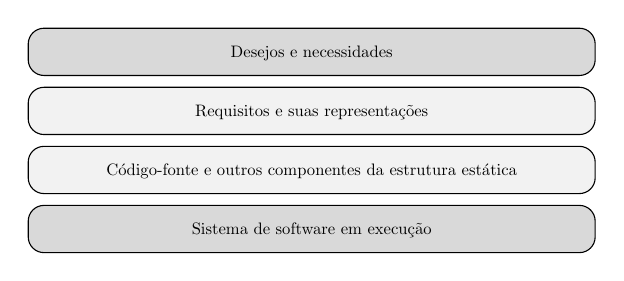
\begin{tikzpicture}[x=1.2cm, y=1.2cm]
  % retangules
  \draw[round,fill=black!15] (1,-1) rectangle (7,-1.5);
  \node at(4,-1.3125) [generation] {Desejos e necessidades};

  \draw[round,fill=black!5] (1,-1.625) rectangle (7,-2.125);
  \node at(4,-1.9375) [generation] {Requisitos e suas representações};

  \draw[round,fill=black!5] (1,-2.250) rectangle (7,-2.750);
  \node at(4,-2.5625) [generation] {Código-fonte e outros componentes da estrutura estática};

  \draw[round,fill=black!15] (1,-2.875) rectangle (7,-3.375);
  \node at(4,-3.1875) [generation] {Sistema de software em execução};
\end{tikzpicture}
\end{document}
